\section{Layout Management}

When confronted with screens of different sizes and pixel densities
pixel accurate layout usually results in disaster. Therefore some good
method of laying out components on the screen is needed.

In most graphical user interfaces widgets are arranged in some grid like
fashion. Distances are often the same for all screens of a single
program. So one would expect, that the process of laying out components
is highly automated. Unfortunately this is not the case. Especially in
the main stream of software development, there is a tendency to change
the notation (XML, JSON) without reducing the overall complexity.

The ui2go solution to component layout is a layout manager, called
\emph{Combigridlayout}. Combigridlayout was heavily inspired by
\href{http://www.miglayout.com/}{MiG-Layout}. It is not as powerful, but
it basically shares the same layout philosophy and there are some
important differences, that give it a quite distinctive flavour.

\begin{enumerate}
\item
  Combigridlayout is very small and easy to port.
\item
  The layout is done using printf-like layout strings.
\item
  Combigridlayout features an easy to use mock-up-mode, that makes it
  possible to test a layout without creating graphical components
  (widgets).
\end{enumerate}

In ui2go Combigridlayout is the basic layout manager, that can be used
for nearly all purposes. Components are laid out like printing lines
onto a piece of paper using the Addf (add formatted) command. Here is a
simple example, that adds a canvas to a window.

\begin{verbatim}
    win := widget.NewWindow()

    canvas := widget.NewCanvas()
    win.Addf("%c growxy", canvas)

    win.Show()
    win.Run()
\end{verbatim}

The layout work is done in the line

\begin{verbatim}
    win.Addf("%c growxy", canvas)
\end{verbatim}

The layout is specified by the layout string \texttt{\%c growxy}.
\texttt{\%c} is a placeholder for the widget. \texttt{growxy} tells the
layout manager to use all available space for the component.

One interesting aspect of the \texttt{Addf} command is the mock-up mode.
It is legal to omit the component parameter. Combigridlayout then
creates a dummy widget to provide a preview of the final layout.

Combigridlayout provides just a few basic layout commands, but in
conjunction with layout containers, that may be arbitrarily nested,
these commands are quite versatile:

\vspace{1em}
\begin{tabular}{lp{9cm}}
Layout Command & Meaning\\[0.5ex]
\%c & Placeholder for a component (widget)\\[0.5ex]
growx & Eat up the available space in x direction. An additional integer
parameter serves as a weight, when there are more than one grow
commands.\\[0.5ex]
growy & Eat up the available space in y direction. An additional integer
parameter serves as a weight, when there are more than one grow
commands.\\[0.5ex]
growxy & Eat up the available space in x and y direction. This command
always comes without a parameter.\\[0.5ex]
spanx & Denotes how many grid cells in x direction are covered by the
component.\\[0.5ex]
spany & Denotes how many grid cells in y direction are covered by the
component.\\[0.5ex]
wrap & Start a new line
\end{tabular}
\vspace{1em}

\pagebreak

\subsection{Border Layout}

This example shows the border layout, that is the basic layout for many
traditional GUI programs.

\begin{figure}[ht]
\centering
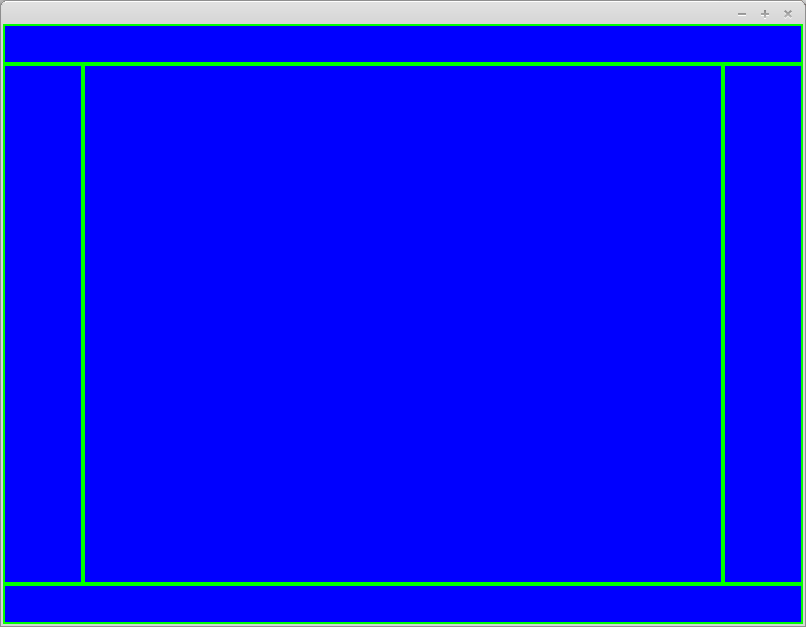
\includegraphics[width=12cm]{img/borderlayout.png}
\caption{Classical border layout.}
\end{figure}

\begin{verbatim}
    win := widget.NewWindow()

    win.Addf("%c spanx 3 wrap")
    win.Addf("%c %c growxy %c wrap")
    win.Addf("%c spanx 3 ")

    win.Show()
    win.Run()
\end{verbatim}

The easiest way to grasp the layout is to scan for the \texttt{\%c}
placeholders. In the above example there are three lines, the first
containing one component, the second containing three components and the
last containing one component.

In the lines with only one component, the component spans three grid
cells (\texttt{spanx 3}). In the second line the middle component eats
up all available space (\texttt{growxy}). So the other components are
made as small as possible.

When creating a new layout it is recommended to first write some lines
containing only \texttt{\%c} and add the constraints thereafter.


\subsection{Grid Layout}

\begin{figure}[ht]
\centering
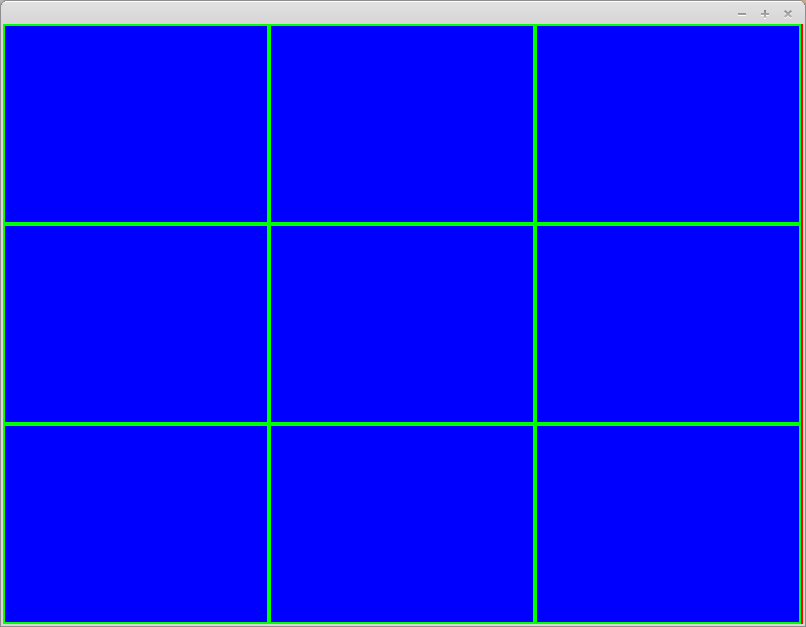
\includegraphics[width=12cm]{img/gridlayout.png}
\caption{Grid layout with equally sized cells.}
\end{figure}

\begin{verbatim}
    win := widget.NewWindow()

    win.Addf("%c growxy %c growx %c growx wrap")
    win.Addf("%c growy  %c       %c wrap")
    win.Addf("%c growy  %c       %c     ")

    win.Show()
    win.Run()
\end{verbatim}

The grid layout is somewhat similar to the border layout, but now there
are three lines containing three widgets. All widgets should be equal in
size. So the \texttt{grow} command is provided. Note, that for some
components \texttt{grow} is not specified. The components automatically
adapt to the grid size, which is already fully specified by other
components.

\pagebreak

\subsection{Classical Input Mask}

\begin{figure}[ht]
\centering
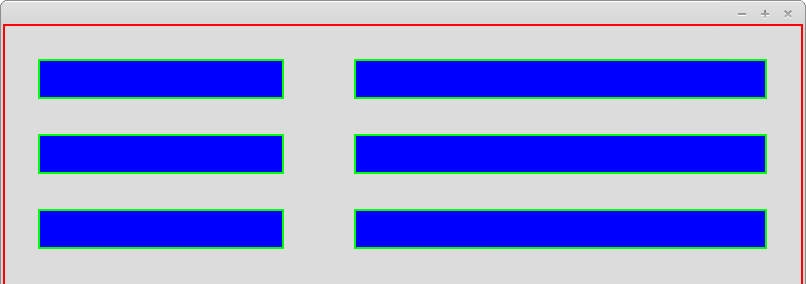
\includegraphics[width=12cm]{img/inputmask.png}
\caption{Mock-up of a traditional input mask.}
\end{figure}

\begin{verbatim}
    win := widget.NewWindow()

    gaps := widget.GridGaps{
        Top:            1,
        Begin:          1,
        End:            1,
        Bottom:         1,
        BetweenColumns: 2,
        BetweenRows:    1}.Unit(widget.Cm)
    win.SetGaps(gaps)

    win.Addf("%c growx 1 %c growx 2 wrap")
    win.Addf("%c         %c         wrap")
    win.Addf("%c         %c")

    win.Show()
    win.Run()
\end{verbatim}

The input mask example features one interesting topic: grid gaps.
Usually distances to the window border and between components are always
the same. So it is easy to specify them for the whole window using
\texttt{SetGaps}.

